%%%%%%%%%%%%%%%%%%%%%%%%%%%%%%%%%%%%%%%%%%%%%%%%%%%%%%%%%%%%%%%%%%%%%%%%%%%%%%
%
% Section file included in main project file using \input{}
%
% Assumes that LaTeX2e macros and packages defined in cg_comp.sty are
%   available
%
%%%%%%%%%%%%%%%%%%%%%%%%%%%%%%%%%%%%%%%%%%%%%%%%%%%%%%%%%%%%%%%%%%%%%%%%%%%%%%

 \section{Tempering the Classical Guitar\label{sct:temp}}

 \begin{quote}
 Temperament: A compromise between the acoustic purity of theoretically exact intervals, and the harmonic discrepancies arising from their practical employment. --- Dr.\ Theo.\ Baker~\cite{ref:baker1895dmt}
 \end{quote}

In \fig{shift_alhambra8p_ej45_fact_temp}, the Alhambra 8P factory guitar with normal tension strings tuned to 12-TET shows the third string having the greatest error in tuning across the fretboard. Tuning the factory guitar to 12-TET exacts a perfect-fifth in the third string while playing a C major chord in first position. This results in the third string being too sharp for the other common chords of E major (G\#), A major and D major (A), particularly when the guitar is played at a higher fret position. One way to reduce this error is by lowering the pitch of the third string below 12-TET with an electronic tuner. Another more comprehensive system is to tune all the strings harmonically to the fifth string, which lowers the third string by 7 cents as well as tempering the remaining strings.

In this particular case, the ``Harmonic Tuning Method'' can be followed using these steps:
 \begin{enumerate}
  \item Begin by tuning the fifth string to A$_2 = 110$~Hz, resulting in a fifth-fret harmonic of A$_4 = 440$~Hz. (This can also be tuned by ear using an A$_4$ tuning fork).
  \item Tune that harmonic to the seventh fret harmonic of the fourth string, which is also A$_4 = 440$~Hz.
  \item Tune the seventh fret harmonic on the fifth string (330~Hz, or 0.37~Hz sharper than 12-TET E$_4$) to the fifth-fret harmonic of the sixth string.
  \item The seventh fret harmonic on the fifth string can tune the remaining fretted strings: the ninth fret on the third string, the fifth fret on the second string, and the open first string.
 \end{enumerate}
 \begin{table}[htbp]
  \centering
  \caption{\label{tbl:harmonic_tuning} Harmonic tuning methodology based on A$_4$ and E$_4$. The asterisk indicates a harmonic with a null at the designated fret.}
    \begin{tabular}{cc}
    \toprule
    Reference String/Fret &  Target String/Fret \\
    \midrule
     A$^\ast$/5 (A$_4$) & D$^\ast$/7 \\
     A$^\ast$/7 (E$_4$) & E$^\ast$/5 \\
     A$^\ast$/7 (E$_4$) & G/9 \\
     A$^\ast$/7 (E$_4$) & B/5 \\
     A$^\ast$/7 (E$_4$) & E/0 \\
    \bottomrule
    \end{tabular}
 \end{table}%
We have summarized these steps in \tbl{harmonic_tuning}, and in \Fig{shift_alhambra8p_ej45_harmonic} we show the same guitar tuned in this fashion. Note that other tuning choices can be made depending on the piece being played. For example, the third string could also be tuned at the second fret to A$_3 = 220$~Hz using the fifth-string harmonic at the 12$^\text{th}$ fret, and/or the first string could be tuned at the fifth fret to A$_4$ using the fifth-fret harmonic of the fifth string. The flexibility of the harmonic tuning method --- and its reliance on only an A$_4$ tuning fork --- is a great asset for the classical guitarist.

% In fact, compensation at the factory and harmonic tuning can be combined to allow guitars with a wide variety of string sets to be well-tempered. For example, in \fig{shift_alhambra8p_ej45_comp_x3}, we plot frequency shifts (in cents) for an ``Alhambra 8P'' guitar with normal tension nylon strings (D'Addario EJ45). But, instead of the factory setbacks, we set $\Delta S$ and $\Delta N$ to the mean of the corresponding column in \tbl{ej45_setbacks} \emph{neglecting the third string}. This choice results in significant reductions in those setbacks, but the RMS frequency error for the third string is 4.7~cents for 12-TET tuning. In \fig{shift_alhambra8p_ej45_harm_x3}, we show that the harmonic tuning method described in \tbl{harmonic_tuning} reduces that RMS error to 2.2~cents.

 \begin{figure}
  \centering
  \begin{subfigure}[b]{0.45\textwidth}
   \centering
   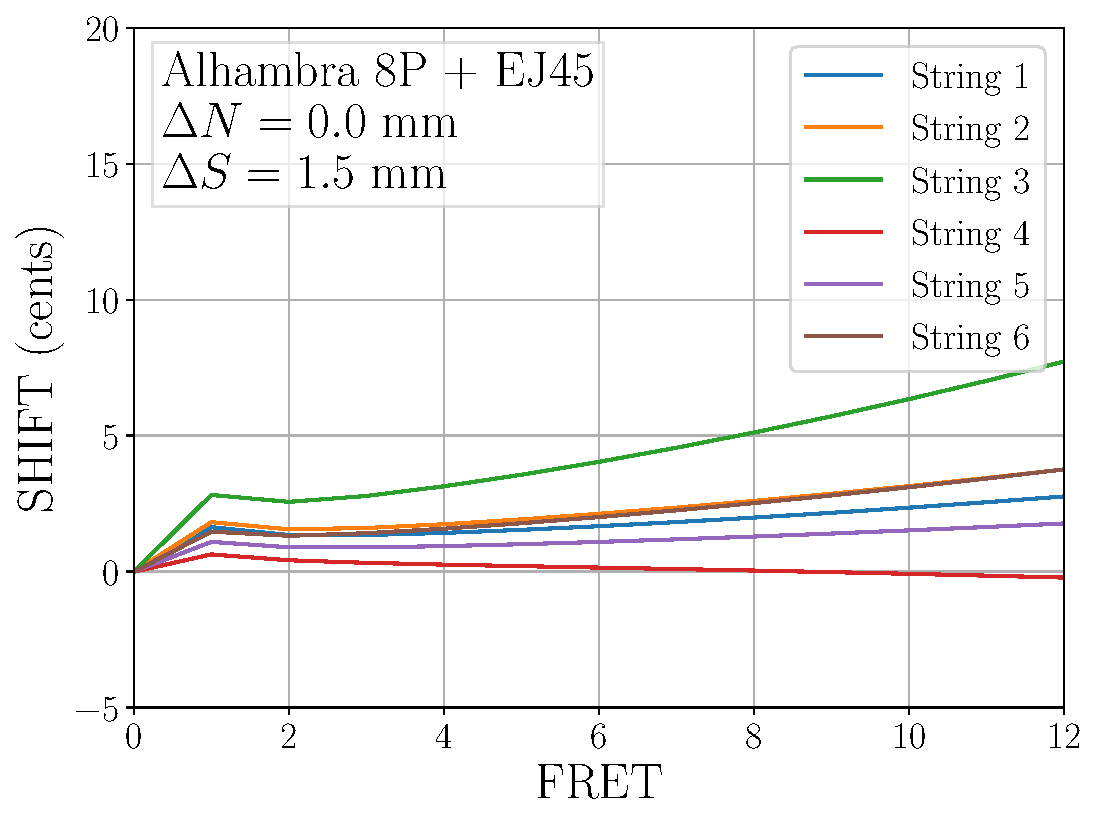
\includegraphics[width=3.25in]{../figures/shift_alhambra8p_ej45_factory}
   \caption{Factory guitar --- 12-TET tuned}
   \label{fig:shift_alhambra8p_ej45_fact_temp}
  \end{subfigure}
  \hspace{0.25in}
  \begin{subfigure}[b]{0.45\textwidth}
   \centering
   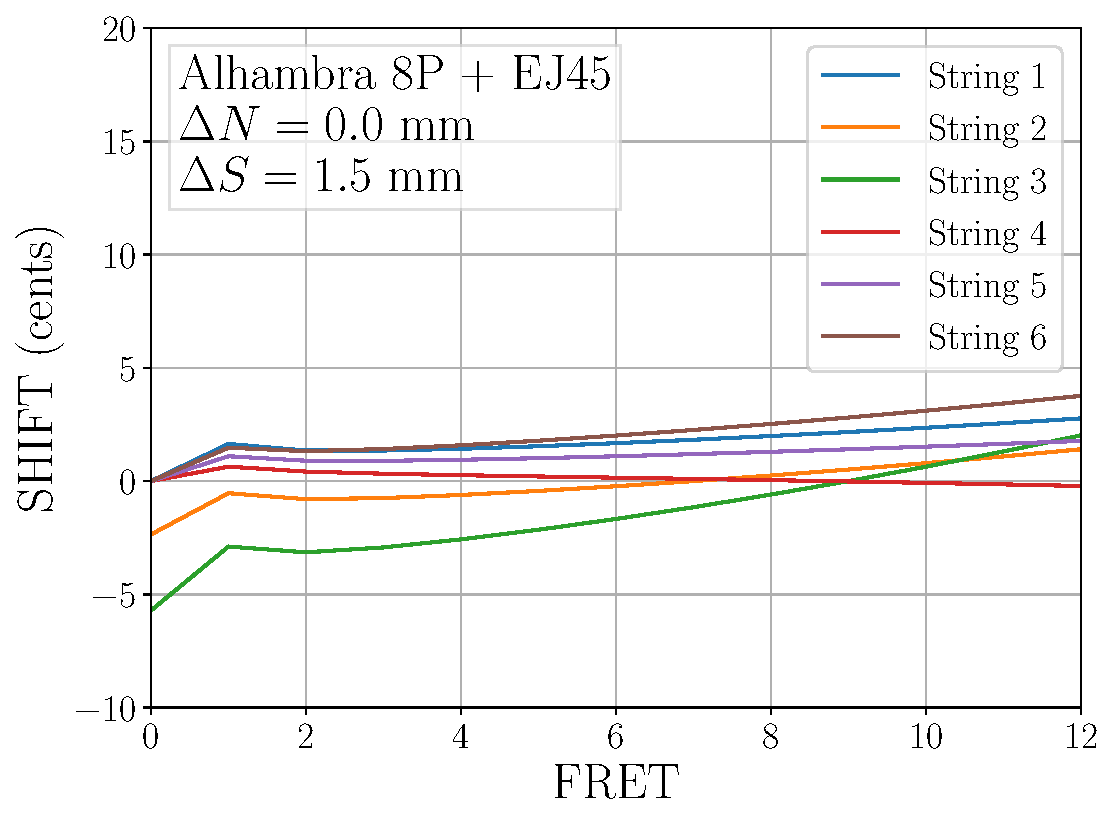
\includegraphics[width=3.25in]{../figures/shift_alhambra8p_ej45_harmonic}
   \caption{Factory guitar --- harmonically tuned}
   \label{fig:shift_alhambra8p_ej45_harmonic}
  \end{subfigure}
  \caption{\label{fig:compensation_alhambra8p_ej45_temp} Frequency shift (in cents) for an Alhambra 8P guitar with normal tension nylon strings (D'Addario EJ45). Here we compare (a) the factory guitar tuned to 12-TET with (b) the same guitar harmonically tuned using the approach outlined in \tbl{harmonic_tuning}.}
 \end{figure}

%  \begin{figure}
%   \centering
%   \begin{subfigure}[b]{0.45\textwidth}
%    \centering
%    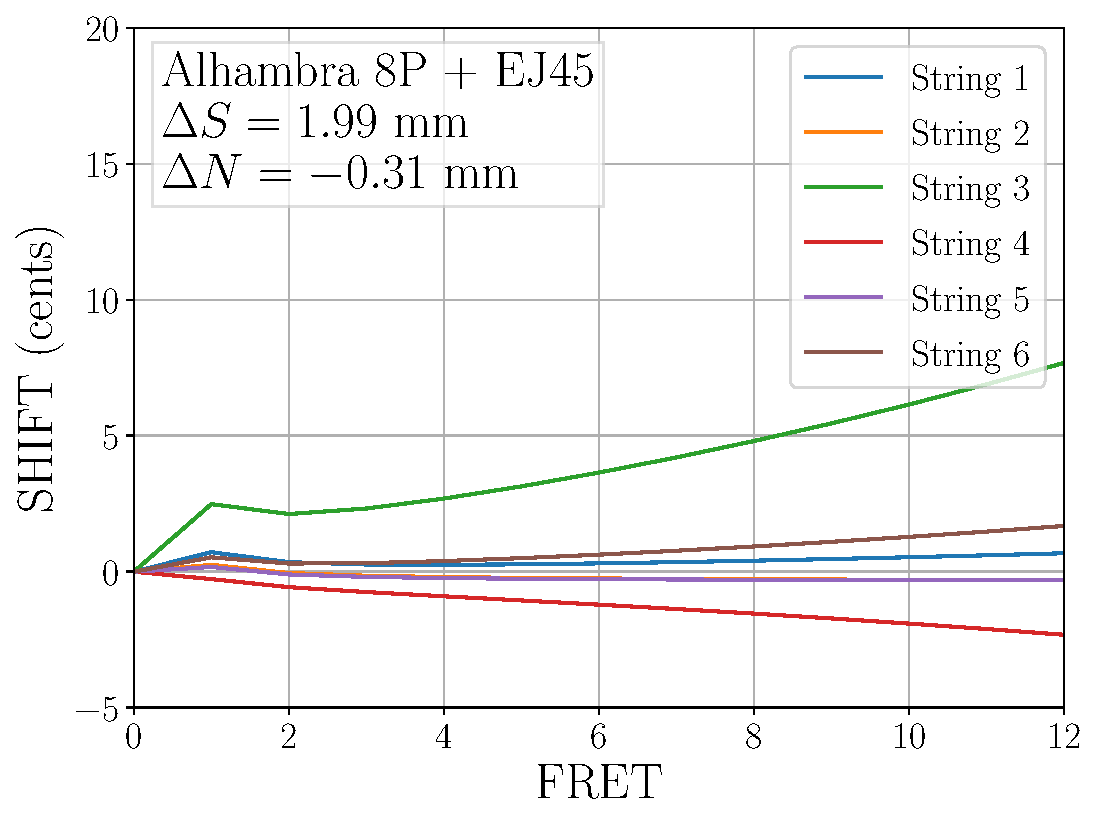
\includegraphics[width=3.25in]{../figures/shift_alhambra8p_ej45_comp_x3}
%    \caption{Compensated guitar --- 12-TET tuned}
%    \label{fig:shift_alhambra8p_ej45_comp_x3}
%   \end{subfigure}
%   \hspace{0.25in}
%   \begin{subfigure}[b]{0.45\textwidth}
%    \centering
%    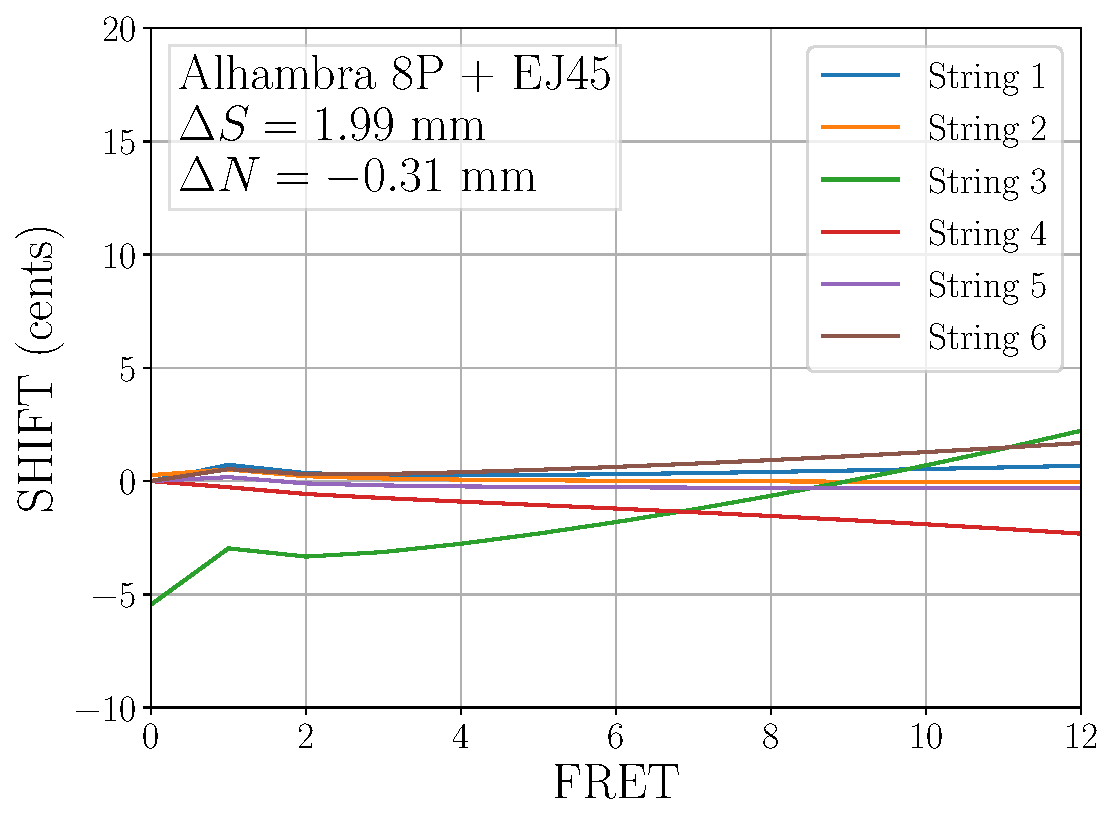
\includegraphics[width=3.25in]{../figures/shift_alhambra8p_ej45_harm_x3}
%    \caption{Compensated guitar --- harmonically tuned}
%    \label{fig:shift_alhambra8p_ej45_harm_x3}
%   \end{subfigure}
%   \caption{\label{fig:compensation_alhambra8p_ej45_x3} Frequency shifts (in cents) for an ``Alhambra 8P'' guitar with normal tension nylon strings (D'Addario EJ45). Instead of the factory setbacks, in (a) we set $\Delta S$ and $\Delta N$ to the mean of the corresponding column in \tbl{ej45_setbacks} \emph{neglecting the third string}. In (b), we show the same guitar harmonically tuned using the approach outlined in \tbl{harmonic_tuning}.}
%  \end{figure}
